\section{Opportunities for reducing exploration cost}
At a high level, \name reduces the exploration cost by leveraging the
insight that the resource-accuracy tradeoffs show substantial spatial
and temporal correlations, which allow us to significantly reduce the
exploration cost by spreading it out across time and over space.

\subsection{Temporal correlation}

To show the temporal correlations of the resource-accuracy tradeoffs, 
we examine the timescales on which the resource-accuracy tradeoffs 
of a configuration change. 
Figure~\ref{??} \jc{shows some results}

Besides a substantial temporal correlation, Figure~\ref{??} also
reveals that at any moment, most configurations are far-from-optimal
and remain so for a sustained period of time.

Inspired by such temporal correlations, we can prune the space of 
configurations by avoiding reprofiling those configurations that have
shown far-from-optimal performance in the near past \Section\ref{??}.

\begin{figure}[h!]
\centering
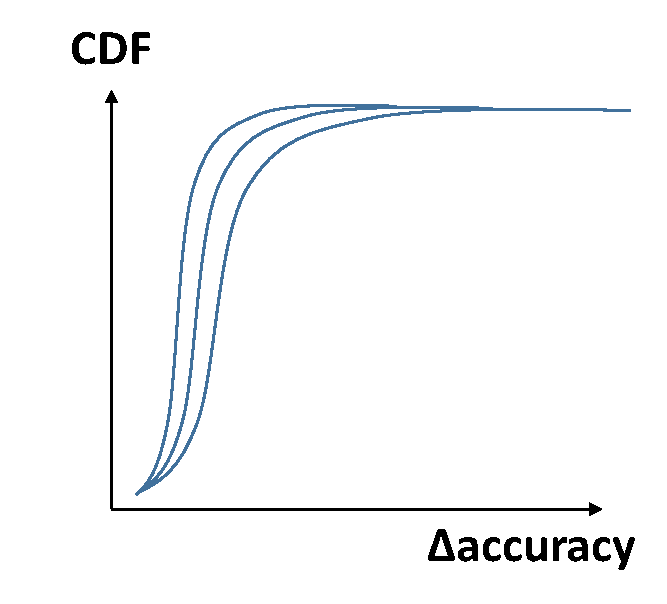
\includegraphics[width=0.3\textwidth]{figures/TemporalCorrelation.pdf}
\vspace{-0.2cm}
\tightcaption{Temporal similarity of \nn accuracy}
\label{fig:TemporalCorrelation}
\end{figure}

\subsection{Spatial correlation}

While leveraging the temporal correlation could greatly reduce the 
cost of exploration per query and video feed, doing adaptive 
profiling for each video feed still bear a non-trivial overhead.
To further trim the exploration cost, we can take advantage of 
the spatial correlations across cameras. 

To show the Figure~\ref{??} shows the distribution of similarity 
between the resource-accuracy tradeoff of the same configuration 
in different video feeds.
\jc{shows some results}

While not all camera feeds are similar, we observe some ``clusters''
of camera feeds. 
A closer look at the cameras in the same cluster shows that they 
often share characteristics such as

\begin{figure}[h!]
\centering
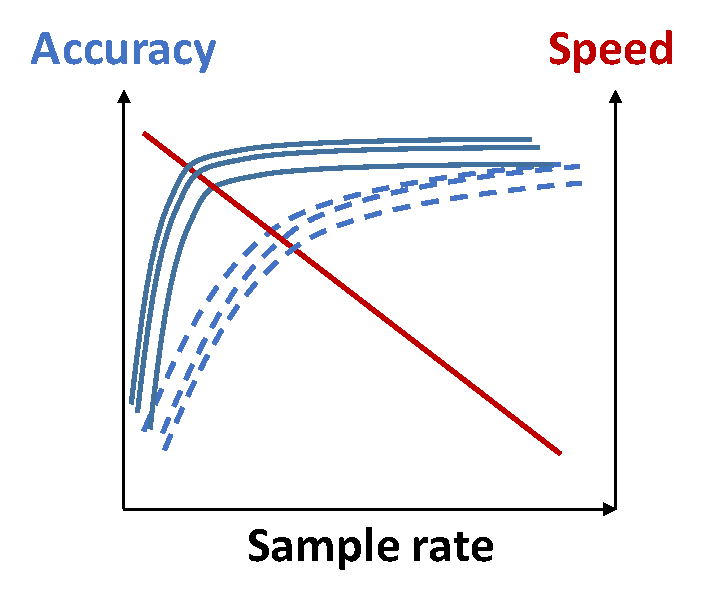
\includegraphics[width=0.3\textwidth]{figures/SpatialCorrelation.pdf}
\vspace{-0.2cm}
\tightcaption{Spatial similarity of \nn accuracy across multiple cameras}
\label{fig:SpatialCorrelation}
\end{figure}
